\chapter{Beleuchtung}

\section{Einführung}
Die Eigenschaften eines Objekts werden bestimmt durch seine Beleuchtungseigenschaften. Das heisst, ein glänzendes Objekt könnte z.B. us Plastik bestehen, ein mattes Objekt aus Ton oder ähnlichen. Konkret sind dies folgende Eigenschaften:
\begin{enumerate}
	\item Farbe
	\item Reflexion
	\item Transparenz
	\item Struktur (matt / glänzend)
	\item Spiegelung
	\item Textur
\end{enumerate}
Nachfolgend werden einige Beleuchtungsmodelle beschrieben. Es wäre zu aufwändig, die physikalisch korrekte Beleuchtung zu berechnen, deswegen nimmt man Vereinfachungen des Beleuchtungsmodells. Nachfolgend werden einige solcher Vereinfachungen dargestellt.
\section{Lambert Beleuchtungsmodell - Diffuse Reflektion}

Bei einem matten Objekt reflektiert die Oberfläche gleichmässig in alle Richtungen. Für die Kamera heisst das nun, dass egal aus welchem Winkel das Objekt betrachtet wird, die Farbe an einem Punkt immer dieselbe sein wird. Diese Farbe an einem Punkt wird also bestimmt durch:
\begin{enumerate}
	\item Farbe des Lichts
	\item Intensität des Lichts
	\item Farbe des Materials
\end{enumerate}
Die Intensität des Lichts ist abhängig vom Winkel, in dem es auftrifft - ist z.B. im Winter ja auch so, dann scheint die Sonne in einem steileren Winkel - und schon wird es kalt.

Formal ausgedrückt ist die Energie einer beleuchteten Fläche proportional zum Cosinus zwischen Lichtrichtung und Flächennormalen.
\begin{displaymath}
I_d = I_L * k_d * cos \phi
\end{displaymath}
wobei 
\begin{displaymath}
cos \phi = \vec{N}*\vec{L}
\end{displaymath}

\begin{description}
	\item[\(\vec{N}\)] Normalvektor der Fläche
	\item[\(\vec{L}\)] Richtung zur Lichtquelle
	\item[\(I_d\)] Reflektierte Intensität
	\item[\(I_L\)] Intensität der Lichtquelle
\end{description}

\section{Phong Modell}
Phong wird für glänzende Reflektionen verwendet. 
\begin{figure}[!ht]
	\centering
	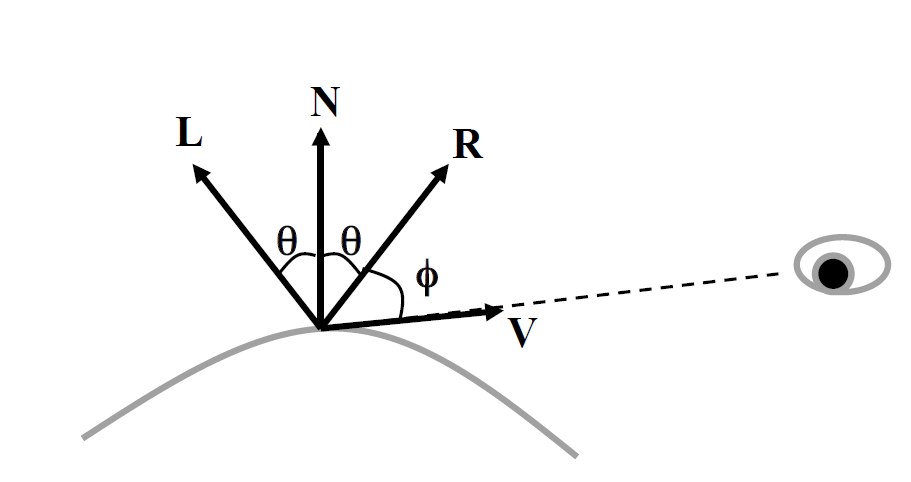
\includegraphics[width=0.4\linewidth]{fig/phong}
	\caption{Phong Beleuchtungsmodell}
	\label{fig:phong}
\end{figure}
Siehe Abbildung \ref{fig:phong} - wir haben eine Fläche eines Objekts. Diese hat einen Normalenvektor - hier \(N\). Das Licht kommt aus der Richtung von \(L\), hat also einen Winkel zum Normalenvektor - hier \(\theta\). Jetzt ist es wie beim Billard - Eintrittswinkel = Austrittswinkel. Wenn wir also nun genau im Reflektionswinkel auf das die Fläche schauen würden, dann hätten wir die volle Reflektion des Objekts. Je weiter wir aber weg sind von diesem \textit{Austrittswinkel} - hier \(R\), desto schwächer wird auch die Reflektion. 

Deswegen können wir folgende Formel aufstellen - die jetzt hoffentlich etwas verständlich ist:
\begin{displaymath}
I_s = I_L*k_s*cos^{n_s}\theta
\end{displaymath}

\begin{description}
	\item[\(I_s\)] Intensität des reflektierten Strahls
	\item[\(I_L\)] Intensität des einfallenden Lichts
	\item[\(k_s\)] Beleuchtungskoeffizient (abhängig davon, wie stark das Objekt welche Farbe reflektiert)
	\item[\(n_s\)] Wie nahe ist die Oberfläche an einer 'ideal reflektierenden'
\end{description}

\begin{figure}[!ht]
	\centering
	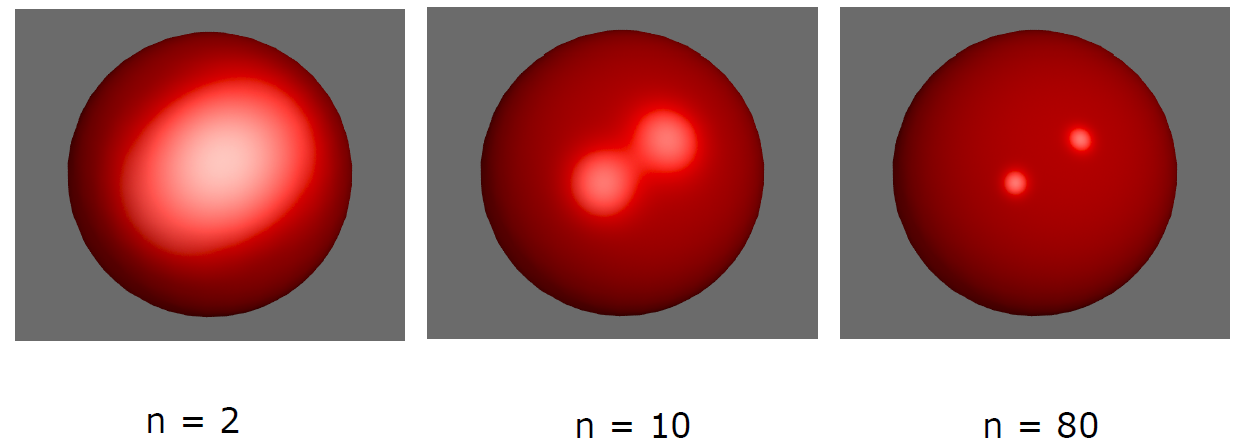
\includegraphics[width=0.4\linewidth]{fig/phong_koeffizienten}
	\caption{Beispiele für verschiedene Werte von \(n_s\)}
	\label{fig:phong_koeffizienten}
\end{figure}

\subsection{Berechnung der Reflektionsrichtung}
Wir haben 2 Vektoren, den Vektor vom einfallenden Licht \(L\) und der Normalenvektor der Fläche \(N\). Ganz wichtig ist es hierbei, dass beide Vektoren \textit{normalisiert} sind, d.h. dass deren Länge (oder Betrag) = 1 ist, sonst funktioniert die folgende Formel nicht und man rechnet mal eine halbe Stunde herum, jaja. Der Reflektionsvektor ist hier dann \(R\).

\begin{displaymath}
R = 2*N(N*L) - L
\end{displaymath}

Die \(*\) bedeuten einfach das Skalarprodukt. Jetzt muss man nur noch den Winkel zwischen dem Vektor \(R\), und dem Vektor der Betrachtung \(V\) herausfinden. Auch hier: beide müssen die Länge 1 haben.
\begin{displaymath}
cos^{-1}(V*R)
\end{displaymath}

Sehr simpel. Um Vektoren übrigens zu normalisieren macht man das:
\begin{displaymath}
V_{normiert} = \frac{V}{|V|}
\end{displaymath}

\(|V|\) ist die Länge (oder der Betrag) des Vektors. Die bestimmt man, wenn man z.B. einen Vektor \((a,b,c)\) hat, so:
\begin{displaymath}
\sqrt{a^2+b^2+c^2}
\end{displaymath}
\section{Abschwächung des Lichts}
In der Physik nimmt die Energie des Lichts mit zunehmender Entfernung quadratisch ab. \(f\) ist hier dann nur ein Faktor, der dann in die Beleuchtungsintensität hineinmultipliziert wird und \(d\) die Distanz
\begin{displaymath}
f = \frac{1}{d^2}
\end{displaymath}
In der Computergrafik sieht das aber doof aus, weil die Lichtintensität zu schnell abnimmt. Besser man nimmt so was:
\begin{displaymath}
\frac{1}{c_1+c_2d+c_3d^2}
\end{displaymath}
Wobei die Faktoren \(c_1 \dots c_n\) frei wählbar sind.


\section{Schattierung}
Wo wird die Beleuchtung überhaupt berechnet?
\subsection{Konstante Schattierung}
Pro Polygon wird nur eine Farbe berechnet - sieht aber dann nicht so schön aus wenn die Objekte gekrümmt sind.
\subsection{Gouraud Schattierung}
Die Farbe wird an den Eckpunkten der Polygone berechnet, die Fläche wird dann linear interpoliert gefüllt.
\subsection{Phong Schattierung}
Hier wird die Beleuchtung für jeden Pixel berechnet, denn hier wird nicht die Farbe sondern der Normalenvektor jeweils innerhalb des Polygons interpoliert. Sieht am schönsten aus.